\documentclass[a4paper, 14pt]{extarticle}

% Поля
%--------------------------------------
\usepackage{geometry}
\geometry{a4paper,tmargin=2cm,bmargin=2cm,lmargin=3cm,rmargin=1cm}
%--------------------------------------


%Russian-specific packages
%--------------------------------------
\usepackage[T2A]{fontenc}
\usepackage[utf8]{inputenc} 
\usepackage[english, main=russian]{babel}
%--------------------------------------

\usepackage{textcomp}

% Красная строка
%--------------------------------------
\usepackage{indentfirst}               
%--------------------------------------             


%Graphics
%--------------------------------------
\usepackage{graphicx}
\graphicspath{ {./images/} }
\usepackage{wrapfig}
%--------------------------------------

% Полуторный интервал
%--------------------------------------
\linespread{1.3}                    
%--------------------------------------

%Выравнивание и переносы
%--------------------------------------
% Избавляемся от переполнений
\sloppy
% Запрещаем разрыв страницы после первой строки абзаца
\clubpenalty=10000
% Запрещаем разрыв страницы после последней строки абзаца
\widowpenalty=10000
%--------------------------------------

%Списки
\usepackage{enumitem}

%Подписи
\usepackage{caption} 

%Гиперссылки
\usepackage{hyperref}

\hypersetup {
	unicode=true
}

%Рисунки
%--------------------------------------
\DeclareCaptionLabelSeparator*{emdash}{~--- }
\captionsetup[figure]{labelsep=emdash,font=onehalfspacing,position=bottom}
%--------------------------------------

\usepackage{tempora}

%Листинги
%--------------------------------------
\usepackage{listings}
\lstset{
  basicstyle=\ttfamily\footnotesize, 
  %basicstyle=\footnotesize\AnkaCoder,        % the size of the fonts that are used for the code
  breakatwhitespace=false,         % sets if automatic breaks shoulbd only happen at whitespace
  breaklines=true,                 % sets automatic line breaking
  captionpos=t,                    % sets the caption-position to bottom
  inputencoding=utf8,
  frame=single,                    % adds a frame around the code
  keepspaces=true,                 % keeps spaces in text, useful for keeping indentation of code (possibly needs columns=flexible)
  keywordstyle=\bf,       % keyword style
  numbers=left,                    % where to put the line-numbers; possible values are (none, left, right)
  numbersep=5pt,                   % how far the line-numbers are from the code
  xleftmargin=25pt,
  xrightmargin=25pt,
  showspaces=false,                % show spaces everywhere adding particular underscores; it overrides 'showstringspaces'
  showstringspaces=false,          % underline spaces within strings only
  showtabs=false,                  % show tabs within strings adding particular underscores
  stepnumber=1,                    % the step between two line-numbers. If it's 1, each line will be numbered
  tabsize=2,                       % sets default tabsize to 8 spaces
  title=\lstname                   % show the filename of files included with \lstinputlisting; also try caption instead of title
}
%--------------------------------------

%%% Математические пакеты %%%
%--------------------------------------
\usepackage{amsthm,amsfonts,amsmath,amssymb,amscd}  % Математические дополнения от AMS
\usepackage{mathtools}                              % Добавляет окружение multlined
\usepackage[perpage]{footmisc}
%--------------------------------------

%--------------------------------------
%			НАЧАЛО ДОКУМЕНТА
%--------------------------------------

\begin{document}

%--------------------------------------
%			ТИТУЛЬНЫЙ ЛИСТ
%--------------------------------------
\begin{titlepage}
\thispagestyle{empty}
\newpage


%Шапка титульного листа
%--------------------------------------
\vspace*{-60pt}
\hspace{-65pt}
\begin{minipage}{0.3\textwidth}
\hspace*{-20pt}\centering

\includegraphics[width=\textwidth]{emblem}
\end{minipage}
\begin{minipage}{0.67\textwidth}\small \textbf{
\vspace*{-0.7ex}
\hspace*{-6pt}\centerline{Министерство науки и высшего образования Российской Федерации}
\vspace*{-0.7ex}
\centerline{Федеральное государственное бюджетное образовательное учреждение }
\vspace*{-0.7ex}
\centerline{высшего образования}
\vspace*{-0.7ex}
\centerline{<<Московский государственный технический университет}
\vspace*{-0.7ex}
\centerline{имени Н.Э. Баумана}
\vspace*{-0.7ex}
\centerline{(национальный исследовательский университет)>>}
\vspace*{-0.7ex}
\centerline{(МГТУ им. Н.Э. Баумана)}}
\end{minipage}
%--------------------------------------

%Полосы
%--------------------------------------
\vspace{-25pt}
\hspace{-35pt}\rule{\textwidth}{2.3pt}

\vspace*{-20.3pt}
\hspace{-35pt}\rule{\textwidth}{0.4pt}
%--------------------------------------

\vspace{1.5ex}
\hspace{-35pt} \noindent \small ФАКУЛЬТЕТ\hspace{80pt} <<Информатика и системы управления>>

\vspace*{-16pt}
\hspace{47pt}\rule{0.83\textwidth}{0.4pt}

\vspace{0.5ex}
\hspace{-35pt} \noindent \small КАФЕДРА\hspace{50pt} <<Теоретическая информатика и компьютерные технологии>>

\vspace*{-16pt}
\hspace{30pt}\rule{0.866\textwidth}{0.4pt}
  
\vspace{11em}

\begin{center}
\Large {\bf Домашняя работа № 2.1} \\ 
\large {\bf по курсу <<Языки и методы программирования>>} \\
\large <<Изучение протокола MQTT>> 
\end{center}\normalsize

\vspace{8em}


\begin{flushright}
  {Студент группы ИУ9-21Б Горбунов А. Д. \hspace*{15pt}\\ 
  \vspace{2ex}
  Преподаватель Посевин Д. П.\hspace*{15pt}}
\end{flushright}

\bigskip

\vfill
 

\begin{center}
\textsl{Москва 2023}
\end{center}
\end{titlepage}
%--------------------------------------
%		КОНЕЦ ТИТУЛЬНОГО ЛИСТА
%--------------------------------------

\renewcommand{\ttdefault}{pcr}

\setlength{\tabcolsep}{3pt}
\newpage
\setcounter{page}{2}

\section{Задание}\label{Sect::task}
    Реализовать на языке JAVA запись и чтение данных в(из) топика в соответствии со своим вариантом:

    Пурвая программа посылает:
    Координаты центров двух окружностей на плоскости и их радиусы.

    Вторая программа принимает данные из первой с помощью mqtt и обраьатывает по правилу:
    1 - если вторая окружность вложена в первую, 0 - в противном случае.

\section{Результаты}\label{Sect::res}

Исходный код программы представлен в листинге~\ref{lst:code1}, ~\ref{lst:code2}

\begin{figure}[!htb]
\begin{lstlisting}[language={java},caption={Publisher.java},label={lst:code1}]
//The code in a more readable form is located in src/Publisher.java
import java.util.Scanner;
import java.lang.Thread;
import org.eclipse.paho.client.mqttv3.*;
import org.eclipse.paho.client.mqttv3.persist.MemoryPersistence;
public class Publisher {
    static String broker = "broker.emqx.io";
    static int port = 1883;
    static String topic = "java/mqtt";
    static String clientId = "java-mqtt-iu9publisher";
    public static void main(String[] args) {
        try {
            MqttClient client = new MqttClient("tcp://" + broker + ":" + port, clientId, new MemoryPersistence());
            client.setCallback(new MqttCallback() {
                public void connectionLost(Throwable throwable) {
                    System.out.println("Connection to MQTT broker lost!");
                }
                public void messageArrived(String s, MqttMessage mqttMessage) throws Exception {
                    System.out.println("Message received:\n\tTopic: " + s + "\n\tMessage: " + new String(mqttMessage.getPayload()));
                }
                public void deliveryComplete(IMqttDeliveryToken MqttDeliveryToken) {  }
            });
            MqttConnectOptions mqttConnectOptions = new MqttConnectOptions();
            mqttConnectOptions.setCleanSession(true);
            System.out.println("Connecting to broker: " + broker);
            client.connect(mqttConnectOptions);
            System.out.println("Connected to MQTT broker!");
            Scanner scanner = new Scanner(System.in);
            while (true) {
                System.out.println("Enter the two centers of circles and their radii in plane:");
                String coordinates = scanner.nextLine();
                MqttMessage mqttMessage = new MqttMessage(coordinates.getBytes());
                mqttMessage.setQos(2);
                mqttMessage.setRetained(false);
                String topic = Publisher.topic;
                System.out.println("Publishing message: " + coordinates);
                client.publish(topic, mqttMessage);
                Thread.sleep(1000);
            }
        } catch (MqttException ex) {
            System.err.println("Exception while connecting to MQTT broker: " + ex.getMessage());
            ex.printStackTrace();
        } catch (InterruptedException ex) {
            System.err.println("Interrupted while publishing messages: " + ex.getMessage());
            ex.printStackTrace();
        }}}
\end{lstlisting}
\end{figure}

\begin{figure}[!htb]
\begin{lstlisting}[language={java},caption={Subscriber.java},label={lst:code2}]
//The code in a more readable form is located in src/Subscriber.java
import org.eclipse.paho.client.mqttv3.*;
import org.eclipse.paho.client.mqttv3.persist.MemoryPersistence;
public class Subscriber {
    static String broker = "broker.emqx.io";
    static int port = 1883;
    static String topic = "java/mqtt";
    static String clientId = "java-mqtt-iu9reader";
    public static void main(String[] args) {
        try {
            MqttClient client = new MqttClient("tcp://" + broker + ":" + port, clientId, new MemoryPersistence());
            client.setCallback(new MqttCallback() {
                @Override
                public void connectionLost(Throwable cause) {
                    System.out.println("Connection lost because: " + cause);   }
                @Override
                public void messageArrived(String topic, MqttMessage message) throws Exception {
                    System.out.println("Received message from topic: " + topic + ", message: " + message.toString());
                    // Extract coordinates from the message
                    String[] coordinates = message.toString().split(", ");
                    double x1 = Double.parseDouble(coordinates[0]);
                    double y1 = Double.parseDouble(coordinates[1]);
                    double x2 = Double.parseDouble(coordinates[2]);
                    double y2 = Double.parseDouble(coordinates[3]);
                    double r1 = Double.parseDouble(coordinates[4]);
                    double r2 = Double.parseDouble(coordinates[5]);
                    int k = 0;
                    double sq = Math.sqrt(Math.pow(x1-x2, 2) + Math.pow(y1-y2, 2));
                    if(sq < r1 && sq + r2 > r1){  k=1;
                    }else if(sq > r1 && sq - r2 < r1){  k=1;  }
                    if(sq == 0 && r1 != r2){   k=0;   
                    }else{k=1;}
                    System.out.println("Is the second circle nested inside the first?:" + k);
                }
                @Override
                public void deliveryComplete(IMqttDeliveryToken token) {        }
            });
            MqttConnectOptions connOpts = new MqttConnectOptions();
            System.out.println("Connecting to broker: " + broker);
            client.connect(connOpts);
            System.out.println("Connected to broker");
            client.subscribe(topic);
            while (true) {  Thread.sleep(1000);   }
        } catch (MqttException | InterruptedException me) {
            System.out.println("Msg: " + me.getMessage());
            System.out.println("Loc: " + me.getLocalizedMessage());
            System.out.println("Cause: " + me.getCause());
            System.out.println("Exception: " + me);
            me.printStackTrace();
        }}}
\end{lstlisting}
\end{figure}

\begin{figure}[!htb]
Результат запуска представлен на рисунке ~\ref{fig:picture_1.png}, ~\ref{fig:picture_2.png}
\end{figure}

\begin{figure}[!htb]
	\centering
	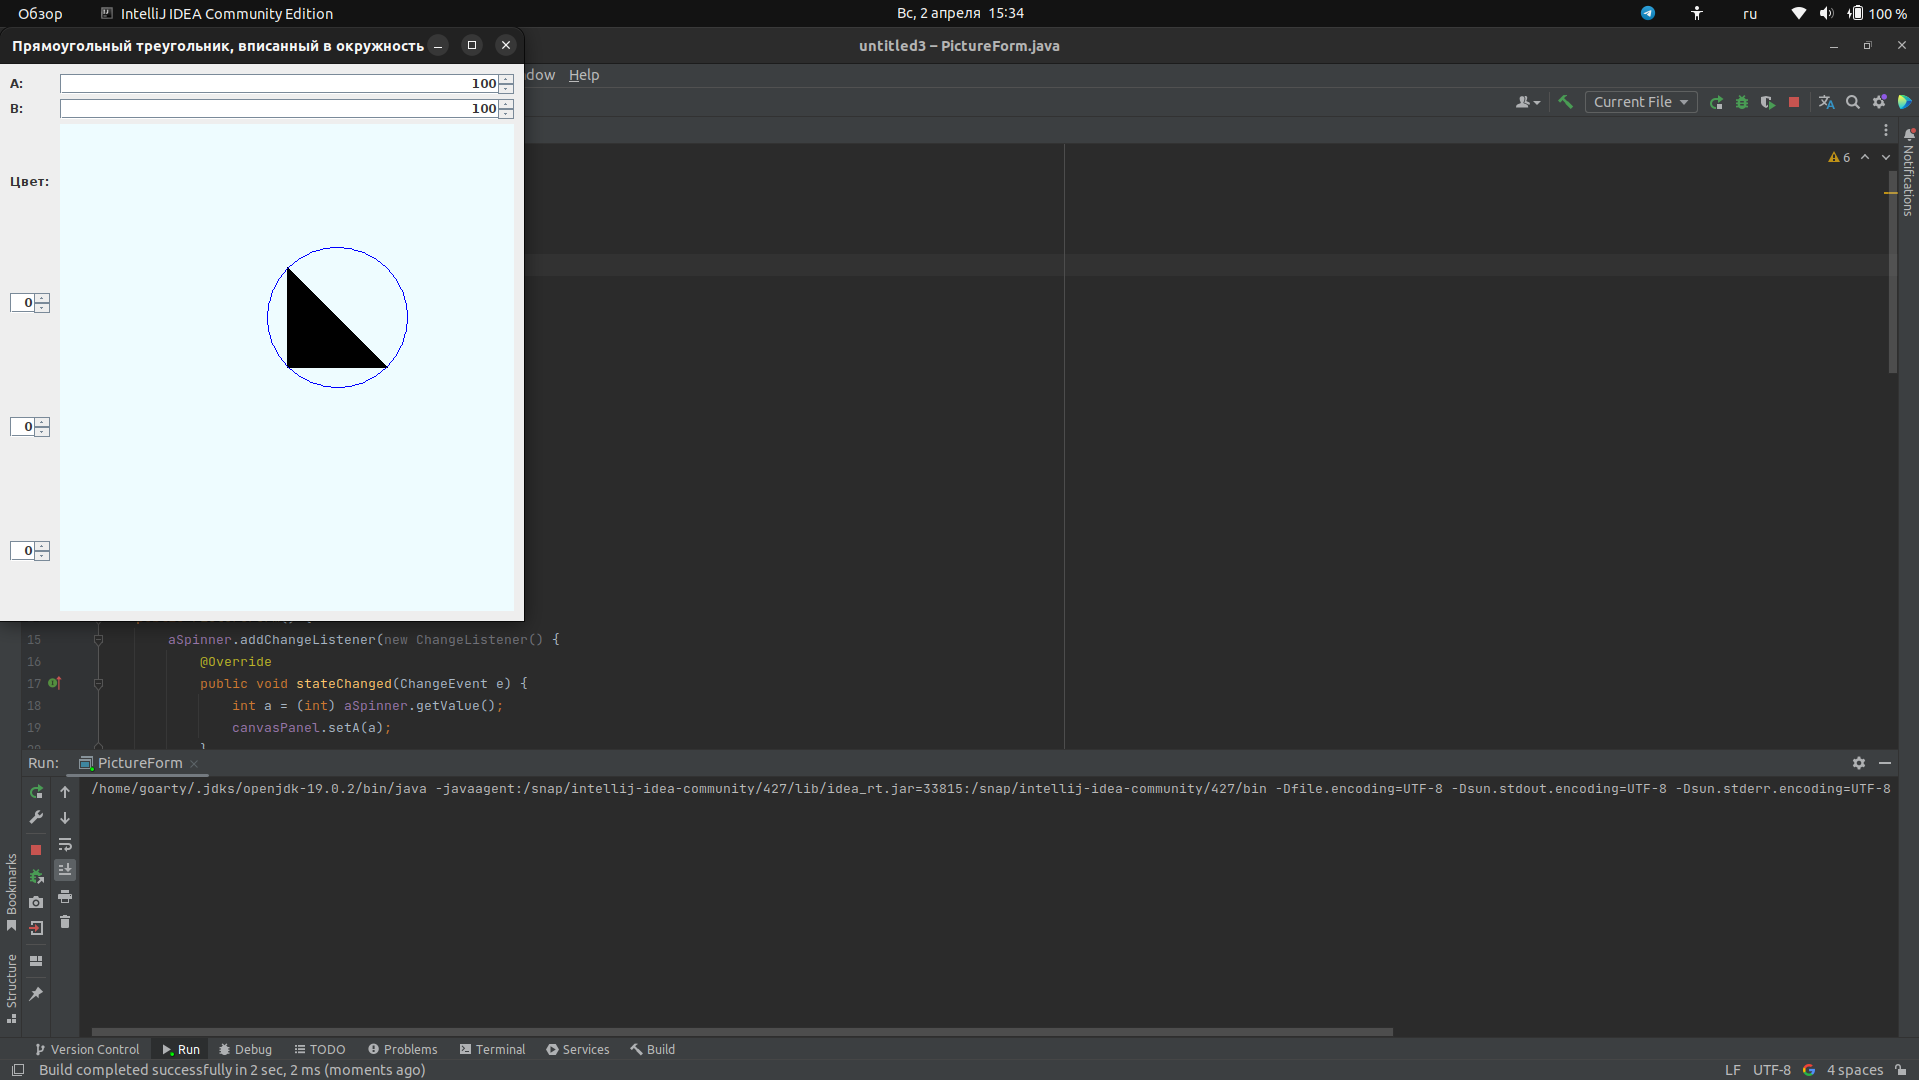
\includegraphics[width=0.8\textwidth]{picture_1.png}
\caption{Реализация Publisher.java}
\label{fig:picture_1.png}
\end{figure}

\begin{figure}[!htb]
	\centering
	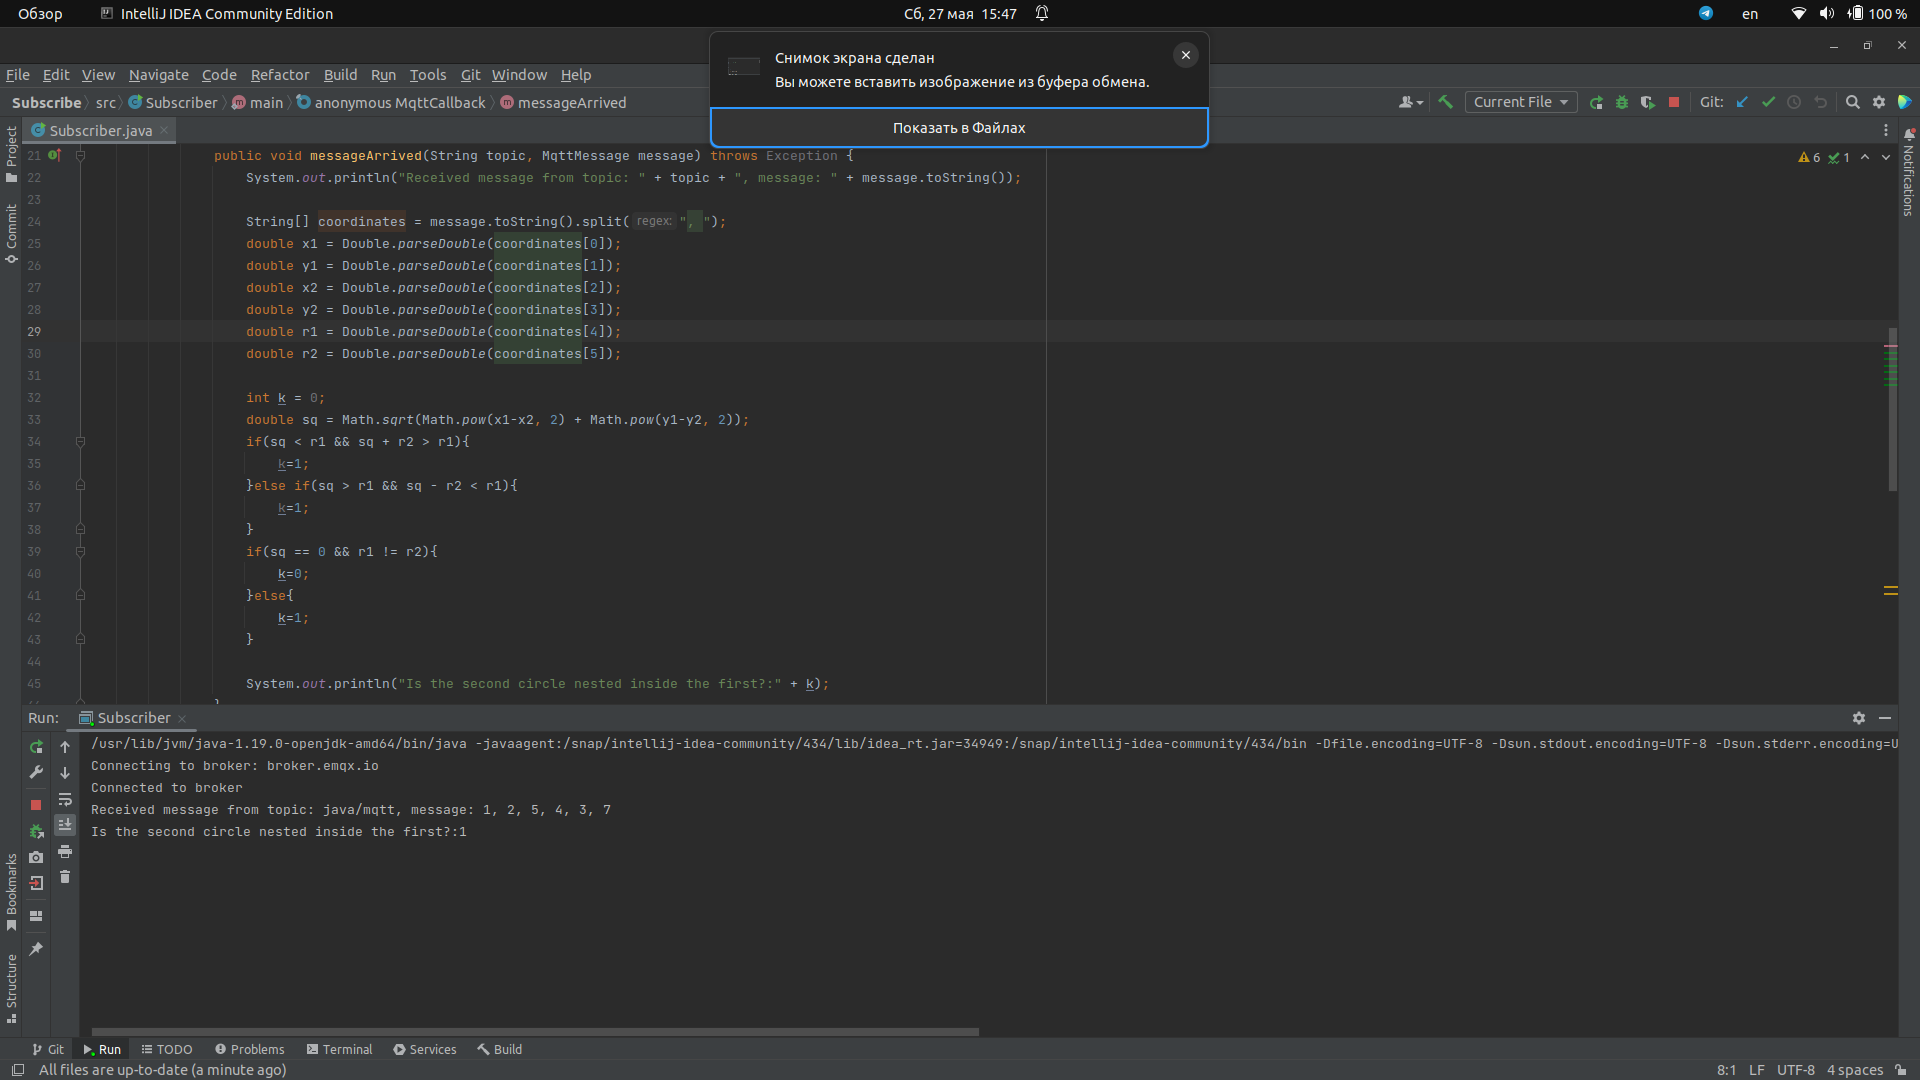
\includegraphics[width=0.8\textwidth]{picture_2.png}
\caption{Реализация Subscriber.java}
\label{fig:picture_2.png}
\end{figure}



\end{document}